\chapter{Funcionamiento de la Solución}
\label{chap:funcionamiento_solucion}

En este capítulo se mostrarán las características principales de la aplicación desarrollada y a modo de referencia para usuarios, mostrando pantallazos de la interfaz, discutiendo las decisiones de diseño de interfaces y experiencia de usuario.\\

Cuando el usuario se conecta por primera vez a la aplicación encontrará la siguiente página de inicio donde este se registrará o autentificará, junto con un video de un demo visual sobre cómo funciona la aplicación.

\begin{figure}[H]
  \centering
  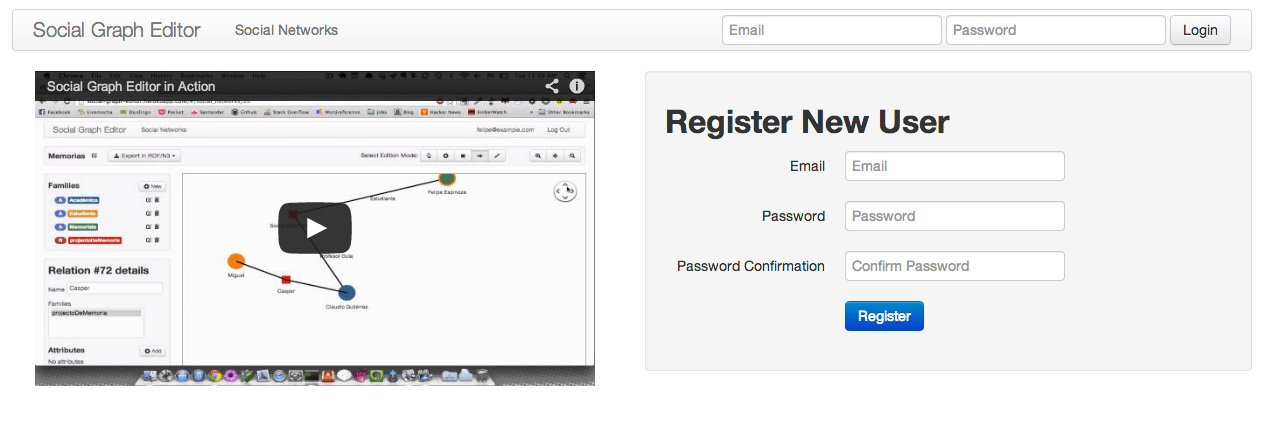
\includegraphics[width=1.0\textwidth]{images/inicio.png}
  \caption[Interfaz de Inicio de La Aplicación]{\emph{Interfaz de Inicio de La Aplicación}. Esta interfaz está pensada para que el usuario se conecte o registre al sitio, junto con entregar un demo en forma de video de como esta aplicación funciona.}
  \label{inicio}
\end{figure}

A continuación se procede a mostrar los principales procesos que se llevan a cabo con la aplicación con sus respectivas interfaces de usuario vistas en detalle.

% 1. qué feature estoy describiendo?
% 2. como funciona? (en términos de uso de la aplicación)
% 3. qué requisito cumple este feature? (hablando de ventajas de este enfoqu)

\section{Registro e Ingreso de Usuarios} % (fold)
\label{sec:registro_e_ingreso_de_usuarios}

Con el fin de mantener la privacidad de las redes sociales que sus usuarios crean, se necesita un sistema de autentificación de usuarios, el cual en este caso requiere una combinación de email y password. Al ingresar a la aplicación por primera vez, el usuario crea su cuenta, es autentificado y redirigido a la página principal donde se muestran sus redes sociales.

% FIXME: check updates
\begin{figure}[H]
  \centering
  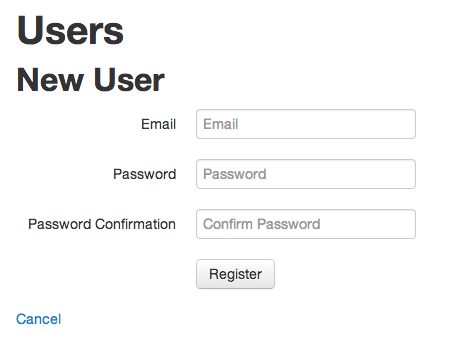
\includegraphics[width=0.6\textwidth]{images/creacion_usuario.png}
  \caption{Formulario de Creación de Usuarios}
  \label{creacion_usuario}
\end{figure}

Cuando el usuario accede de nuevo a la aplicación, esta vez en lugar de registrar un usuario debe autentificarse de modo de acceder a su información vía este pequeño formulario.

% FIXME: check updates
\begin{figure}[H]
  \centering
  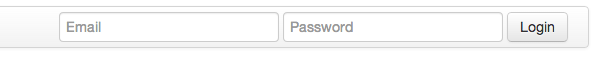
\includegraphics[width=0.7\textwidth]{images/login.png}
  \caption[Formulario de Ingreso]{\emph{Formulario de Ingreso}. Con una combinación de email y password el usuario de autentifica en el sistema.}
  \label{login}
\end{figure}

% section registro_e_ingreso_de_usuarios (end)

% ### 5.2 creación de redes sociales [screenshot]
\section{Creación de Redes Sociales} % (fold)
\label{sec:creacion_de_redes_sociales}

Dado que el usuario registró una cuenta en la aplicación, esta habilitado para crear una red social, inicialmente en la pantalla principal de redes sociales, presiona el botón \emph{Add Social Network} con el cual aparece el formulario de creación que es para darle un nombre y una descripción a la red social como detalles de esta.

% FIXME: check updates
\begin{figure}[H]
  \centering
  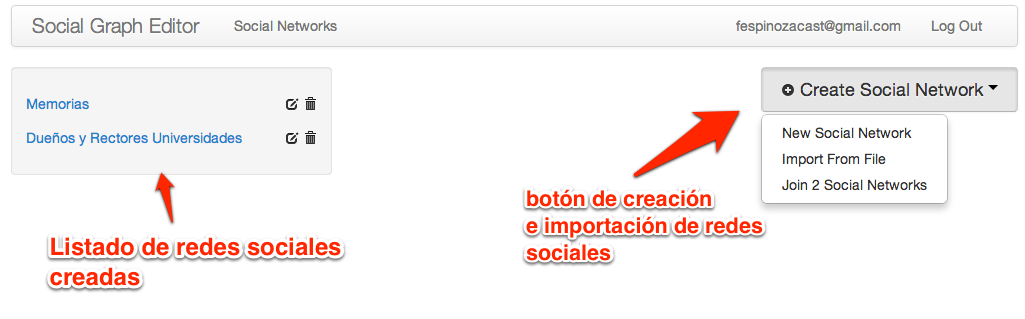
\includegraphics[width=1.0\textwidth]{images/principal_social_networks.png}
  \caption[Pantalla Principal de Redes Sociales]{\emph{Pantalla Principal de Redes Sociales}. Es la primera página luego de que el usuario se autentifica, la cual le permite crear redes sociales para luego complementar su información.}
  \label{principal_social_network}
\end{figure}

% FIXME: check updates
\begin{figure}[H]
  \centering
  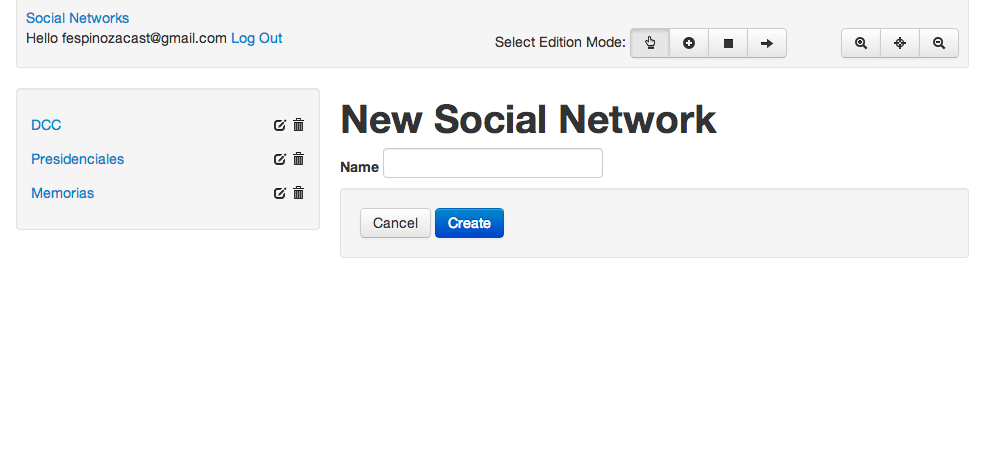
\includegraphics[width=1.0\textwidth]{images/new_social_network.png}
  \caption{Formulario Nueva Red Social}
  \label{new_social_network}
\end{figure}

Esta información ingresada de la red social sirve como detalles de la misma y puede ser editada en cualquier momento, sin embargo, lo más relevante de la creación de la red, es la adición de contenido a la estructura de esta, lo que se cubrirá en la siguiente sección.

% section creación_de_redes_sociales (end)

\section{Edición de Redes Sociales} % (fold)
\label{sec:edicion_de_redes_sociales}

Una vez que el usuario tiene su cuenta y creó una red social, está listo para ir agregando los datos relevantes a sus redes sociales, haciendo click sobre el link con el nombre de la red social recién creada.

\begin{figure}[H]
  \centering
  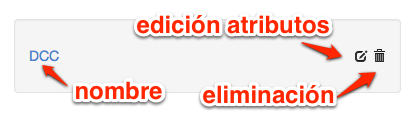
\includegraphics[width=0.5\textwidth]{images/lista_redes_sociales.png}
  \caption[Lista de Redes Sociales]{\emph{Lista de Redes Sociales}. En este lugar aparecen las redes sociales creadas, donde el nombre llega a la edición del contenido de esta, además de contar en el costado con botones para editar sus detalles o eliminar la red.}
  \label{lista_redes_sociales}
\end{figure}

\subsection{Área de Edición de Redes Sociales} % (fold)
\label{sub:area_de_edicion_de_redes_sociales}

El área de edición de redes sociales consiste básicamente de 4 elementos: el canvas donde se crea el grafo de la red social (1), una barra de herramientas para la edición (2), un área donde se definen las familias de actores y relaciones (3) y un formulario con los detalles de las entidades seleccionadas (4).

\begin{figure}[H]
  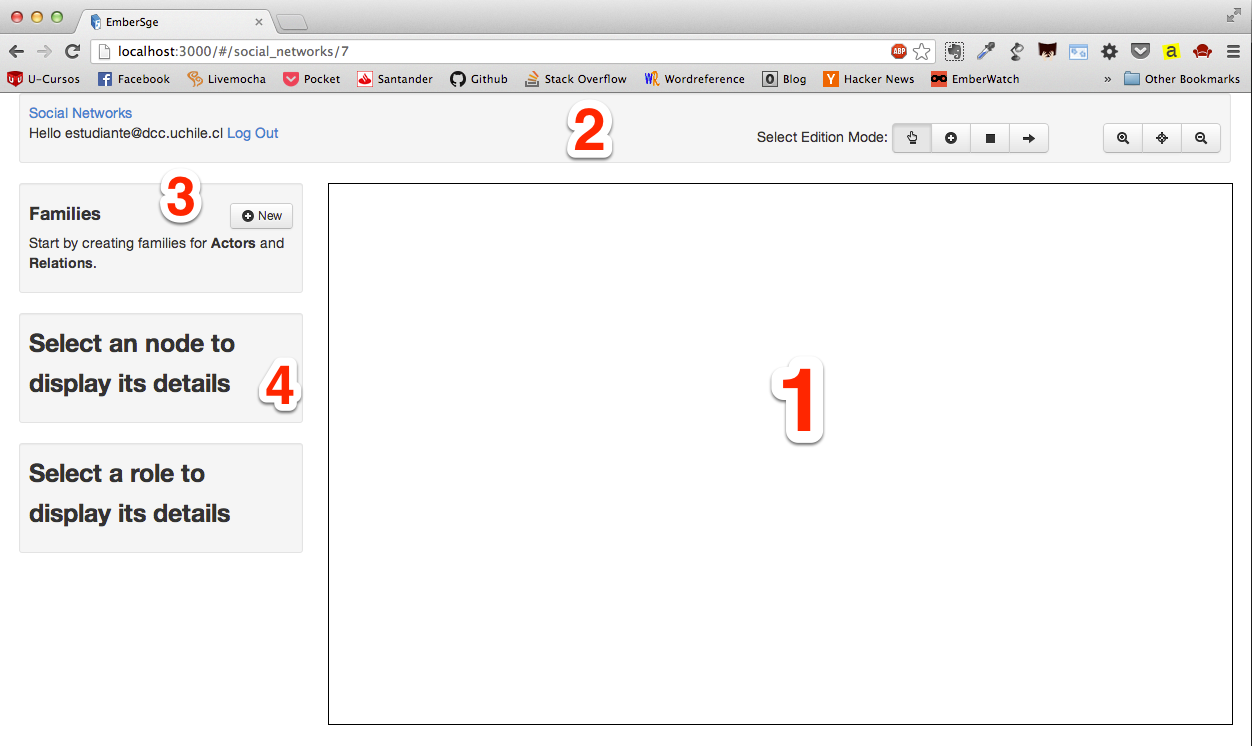
\includegraphics[width=1.0\textwidth]{images/area_edicion_redes.png}
  \caption[Área de Edición de Redes]{\emph{Área de Edición de Redes}. Esta es el área principal donde el usuario completa y manipula la información de las redes sociales creadas, con números para la explicación de las diversas secciones de esta interfaz.}
  \label{area_edicion_redes}
\end{figure}

Esta interfaz está pensada para tener la menor cantidad de elementos posibles, haciendo énfasis en las herramientas primordiales necesarias para la edición del grafo.

\subsubsection{Modos de Edición} % (fold)
\label{ssub:modos_de_edicion}

Para la zona de edición se cuenta con 4 modos de edición, de acuerdo a los cuales puedo realizar acciones diversas cuando hago click dentro de la zona del canvas.

% FIXME: check updates
\begin{figure}[H]
  \centering
  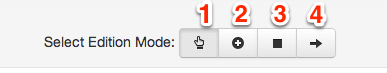
\includegraphics[width=0.6\textwidth]{images/modos_edicion.png}
  \caption[Modos de Edición]{\emph{Modos de Edición}. Botones para seleccionar el modo de edición, con números para explicar los diversos modos.}
  \label{modos_edicion}
\end{figure}

Los modos existentes son:

  \begin{enumerate}
    \item \textbf{Herramienta de Movimiento}: esta herramienta me permite cambiar la posición de los nodos dentro del canvas a voluntad, además de al hacer click en estos seleccionarlos para la edición de sus detalles.
    \item \textbf{Modo Actor}: en este modo, al hacer click en algún punto del canvas creará un nuevo actor dentro de esta en la posición donde se especificó haciendo click. El enfoque será puesto automáticamente en el formulario de detalles del nuevo actor para rellenar rápidamente sus campos necesarios y confirmar la creación del nuevo actor.
    \item \textbf{Modo Relación}: en este modo, al hacer click en algún punto del canvas creará una nueva relación situada en esas coordenadas. El enfoque será puesto automáticamente en el formulario de edición de la relación, pero a diferencia de los actores, las relaciones son automáticamente guardadas al momento de ser creadas y cambian al \emph{modo Rol}.
    \item \textbf{Modo Rol}: en este modo, al momento de hacer click en un actor (manteniendo el botón presionado), puedo arrastrar una flecha y situarla sobre una relación, donde al soltar el botón del mouse, creará automáticamente un nuevo rol del actor seleccionado en la relación seleccionada, para después editar sus detalles en el formulario de roles correspondiente. Además, puedo repetir esta acción cuantas veces sea necesario.
    \item \textbf{Modo Unión de Nodos}: en este modo, al arrastrar un nodo (actor o relación) sobre otro del mismo tipo provocará la aparición de un cuadro de confirmación de la unión entre nodos, que de ser confirmada hará que se unan todas las propiedades de estos en uno solo, en caso contrario el nodo arrastrado retornará a su posición original.
  \end{enumerate}

% subsubsection modos_de_edición (end)

% subsection área_de_edición_de_redes_sociales (end)

\subsection{Creación y Edición de Familias} % (fold)
\label{sub:creacion_y_edicion_de_familias}

Para poder agrupar los nodos (actores y relaciones) dentro de familias, hay un área reservada para la creación propia de estas familias dentro de la red, en donde a continación se explican las principales operaciones con familias dentro de una red social.\\

\begin{figure}[H]
  \centering
  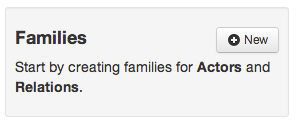
\includegraphics[width=0.6\textwidth]{images/area_familias.png}
  \caption[Área de Familias]{\emph{Área de Familias}. Detalle del área donde se crean las familias en una red social.}
  \label{area_familias}
\end{figure}

Para crear una familia se presiona el botón \emph{New} en la sección de familias, con lo que aparece un formulario con el siguiente:

% FIXME: check updates
\begin{figure}[H]
  \centering
  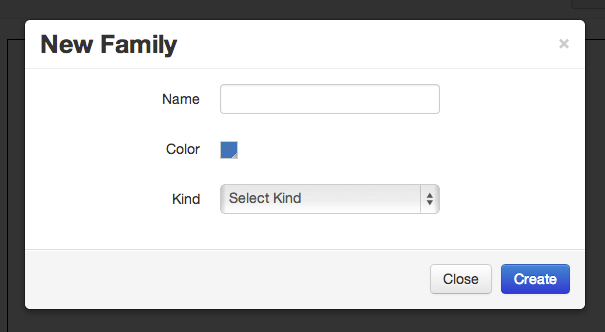
\includegraphics[width=0.7\textwidth]{images/edicion_familias.png}
  \caption[Formulario de Edición de Familias]{\emph{Formulario de Edición de Familias}. Formulario por el cual se define el nombre, color y tipo de familia.}
  \label{edicion_familias}
\end{figure}

Acá se rellena el nombre y se selecciona el color para mostrar los nodos de esta familia y el tipo de nodos a los cuales se les asignará esta familia.\\

Una vez creada, se muestra la familia en el listado con un ícono de \emph{A} para el caso de familias de actores y de \emph{R} en el caso de familias de relaciones. Donde puedo editar sus detalles o eliminarlas con los botones que se encuentran a su lado.

\begin{figure}[H]
  \centering
  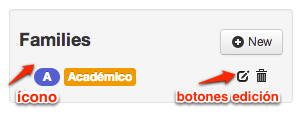
\includegraphics[width=0.5\textwidth]{images/familia_creada.png}
  \caption[Detalle Familia Creada]{\emph{Detalle Familia Creada}. Un ejemplo de una familia creada, con su ícono que indica si corresponde a familia de Actores o Relaciones, además de sus botones de edición y eliminación.}
  \label{familia_creada}
\end{figure}

Es importante destacar, que se puede presionar cualquier tipo de familia, en donde al hacer esto, se cambiará al \emph{modo Actor} o \emph{modo Relación} según corresponda y a continuación cuando creo un actor o relación, por defecto pertenecerá a la familia seleccionada.

% subsection creación_y_edición_de_familias (end)

\subsection{Creación y Edición de Actores} % (fold)
\label{sub:creacion_y_edicion_de_actores}

Para crear actores, se debe definir el modo de edición a \emph{modo Actor}~\ref{ssub:modos_de_edicion}, y hacer click en el canvas donde aparecerá un actor en dicho punto y se enfocará automáticamente el formulario de creación del actor.\\

% FIXME: check updates
\begin{figure}[H]
  \centering
  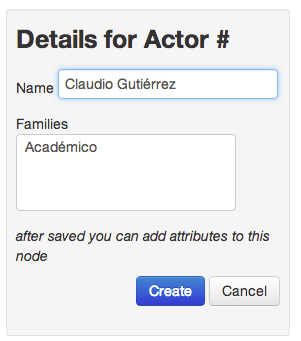
\includegraphics[width=0.5\textwidth]{images/creacion_actor.png}
  \caption{Formulario de Creación de Actor}
  \label{creacion_actor}
\end{figure}

En este formulario se puede rellenar el nombre (opcionalmente), seleccionar las familias a las que pertenece el actor para finalmente confirmar la creación. Luego de esto, la información visual del actor es actualizada, mostrando al actor del color de la(s) familia(s) a la cual pertenece, además de un borde indicando de que es dicho actor el que está seleccionado en este momento.\\

\begin{figure}[H]
  \centering
  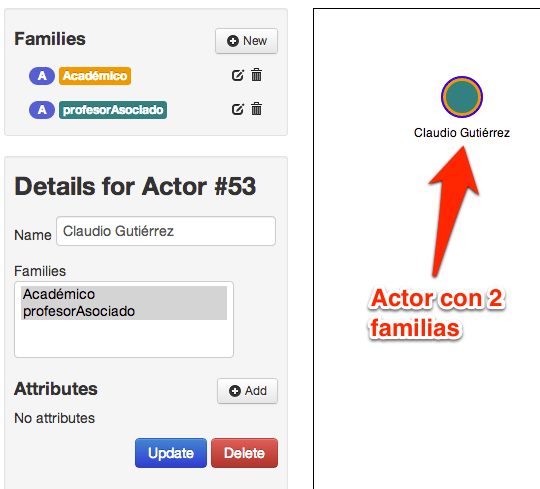
\includegraphics[width=0.6\textwidth]{images/ejemplo_actor_2_familias.png}
  \caption[Ejemplo Actor con 2 Familias]{\emph{Ejemplo Actor con 2 Familias}. Un actor con 2 familias tendrá un círculo con 2 colores de sus familias correspondientes.}
  \label{ejemplo_actor_2_familias}
\end{figure}

El actor puede ser editado en cualquier momento vía el formulario de actor, luego se presiona el botón de actualizar para persistir los cambios, o puede ser eliminado con el botón de borrar, después de confirmar en el cuadro de diálogo 
que aparece.

\begin{figure}[H]
  \centering
  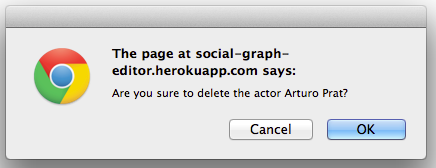
\includegraphics[width=0.5\textwidth]{images/dialogo_eliminacion_actor.png}
  \caption{Diálogo de Eliminación de Actor}
  \label{dialogo_eliminacion_actor}
\end{figure}

% subsection creación_y_edición_de_actores (end)

\subsection{Creación y Edición de Relaciones} % (fold)
\label{sub:creacion_y_edicion_de_relaciones}

Para crear una relación, se debe seleccionar el \emph{modo Relación}~\ref{ssub:modos_de_edicion}, posteriormente hacer click dentro del canvas en donde aparecerá la nueva relación y se mostrará el formulario de edición de la relación. A diferencia de los actores, las relaciones son creadas automáticamente, lo cual cambiará al modo de edición de roles, para agregar los roles correspondientes a la relación sin perder el contexto.

% FIXME: check updates
\begin{figure}[H]
  \centering
  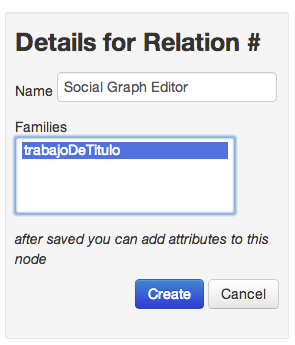
\includegraphics[width=0.5\textwidth]{images/creacion_relacion.png}
  \caption{Formulario de Creación de Relación.}
  \label{creacion_relacion}
\end{figure}

Las relaciones pueden o no tener un nombre, además de pertenecer a una familia, lo que generalmente denota el tipo de relación con la cual se está trabajando, ej: estudiaEn, dueñoDe, etc.\\

La relación puede ser editada en cualquier momento vía el formulario y presionando el botón de actualizar, o eliminada con el botón de borrar, luego de confirmar el cuadro de dialogo que aparece.

% subsection creación_y_edición_de_relaciones (end)

\subsection{Creación y Edición de Atributos en Nodos} % (fold)
\label{sub:creacion_y_edicion_de_atributos_en_nodos}

Una vez teniendo actores y relaciones creados dentro de la red social, es posible agregarles todos los atributos que se estimen conveniente por medio del formulario de edición de actores o relaciones, para esto, en la subsección de atributos en dicho formulario se puede agregar uno presionando el botón \emph{Add}, en donde puedo ingresar un atributo como un par key-value, por ejemplo puedo agregar el atributo \emph{Edad} (key) con el valor \emph{24} a un actor.

% FIXME: check updates
\begin{figure}[H]
  \centering
  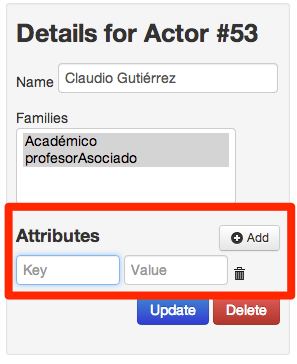
\includegraphics[width=0.5\textwidth]{images/insercion_atributos.png}
  \caption[Añadiendo Atributos a un Actor]{\emph{Añadiendo Atributos a un Actor}. Se presiona el botón Add y luego se puede agregar el nuevo atributo como un par Key Value.}
  \label{insercion_atributos}
\end{figure}

Para editar atributos, se pueden editar directamente en sus campos y luego presionar el botón \emph{Update} para que los cambios sean persistentes, o borrar un atributo presionando el ícono junto a la definición del mismo.

% subsection creación_y_edición_de_atributos_en_nodos (end)

\subsection{Creación y Edición de Roles} % (fold)
\label{sub:creacion_y_edicion_de_roles}

Los roles representan la participación de un actor en una relación, dicha participación o rol, puede tener un nombre o no. Un ejemplo del último caso: en una relación de amistad entre dos personas, puede haber un tercer actor que fue quien los presentó, pero nuevamente, el nombre de un rol es opcional. Para crear un rol, se debe seleccionar el modo de edición de roles~\ref{ssub:modos_de_edicion}, luego con el mouse, pincho un actor y arrastro el mouse hacia una relación, al soltar el mouse el rol va a ser creado inmediatamente y el foco va a ser puesto dentro del formulario de edición del rol.

% FIXME: check updates
\begin{figure}[H]
  \centering
  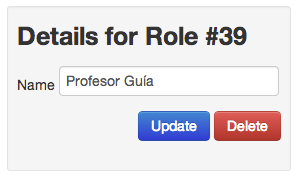
\includegraphics[width=0.5\textwidth]{images/edicion_rol.png}
  \caption[Formulario de Edición de Rol]{\emph{Formulario de Edición de Rol}. En caso de ser necesario, se puede agregar un nombre al rol o eliminarlo desde aquí.}
  \label{edicion_rol}
\end{figure}

En este formulario puedo actualizar el nombre del rol o de ser necesario eliminar el rol. Es importante mencionar que los roles sólo serán creados desde un \emph{Actor} hacia una \emph{Relación}, cualquier otra combinación no resultará en la creación de un rol.

% subsection creación_y_edición_de_roles (end)

% section edición_de_redes_sociales (end)

\section{Exportación en RDF} % (fold)
\label{sec:exportacion_en_rdf}

Como primer paso en la integración de la aplicación con la web semántica, esta permite una exportación de las redes sociales modeladas en formato RDF/N3. Con este fin, se usa la estructura de triples descrita en el modelo de Mauro en la subsección~\ref{sub:representacion_como_triples}. Entonces, para exportar la información de la red social en este formato puede hacerse vía el botón \emph{Export in RDF/N3} en el menú de edición de redes sociales.\\

% FIXME: check updates
\begin{figure}[H]
  \centering
  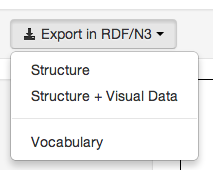
\includegraphics[width=0.4\textwidth]{images/export_button.png}
  \caption[Botón de Exportación de la Red Social]{\emph{Botón de Exportación de la Red Social}. Con este botón se puede exportar en formato RDF/N3: la estructura de la red social, la estructura más la información visual de la red o el vocabulario de esta red.}
  \label{export_button}
\end{figure}

Por ejemplo, podemos tener el caso de una red social como la de la figura~\ref{mini_red_ejemplo}:

% FIXME: check updates
\begin{figure}[H]
  \centering
  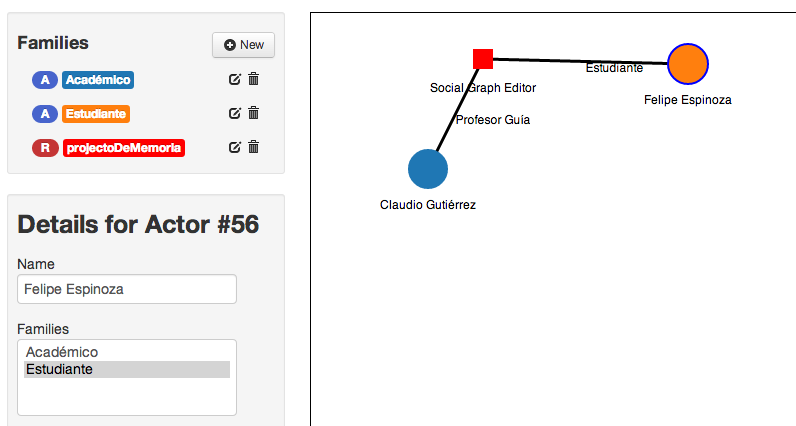
\includegraphics[width=0.8\textwidth]{images/mini_red_ejemplo.png}
  \caption[Micro Ejemplo de Red Social]{\emph{Micro Ejemplo de Red Social}. Una red social que muestra la relación de un estudiante con su profesor guía.}
  \label{mini_red_ejemplo}
\end{figure}


Exportando la estructura únicamente de esta red social, que contiene 2 actores y una relación, se obtendría el siguiente resultado\\

% FIXME: check updates
\lstinputlisting[caption=Exportación RDF red social figura~\ref{mini_red_ejemplo}, style=rdf]{extra/exportacion.n3}
\label{lst:red_n3}

Esta representación RDF/N3 está validada~\cite{validador_rdf}. Es importante mencionar que para dicha representación RDF se define una ontología propia de la aplicación, que cuenta con las definiciones comunes de la aplicación, como por ejemplo Actores, Relaciones y Roles, pero además cuenta con las definiciones de elementos propios de la red como Atributos definidos en esta. El vocabulario correspondiente de la red sería el siguiente:.

% FIXME: check updates
\lstinputlisting[caption=Vocabulario red social figura~\ref{mini_red_ejemplo}, style=rdf]{extra/vocabulary.n3}
\label{lst:vocabulario_n3}

Además en caso de ser necesario, como se menciona antes, se puede exportar agregando la información gráfica de la red social, en donde se incluyen las posiciones de los nodos en el canvas, los colores de las familias definidas, etc.

% section exportacion_en_rdf (end)

\section{Importación en RDF} % (fold)
\label{sec:importacion_en_rdf}

Junto con la exportación en formato RDF que usa la aplicación, esta tiene la funcionalidad de importar a partir de un archivo RDF de la red social como el definido en el ejemplo de código~\ref{lst:red_n3}, para crear una red social a partir de lo importado.

% FIXME: check updates
\begin{figure}[H]
  \centering
  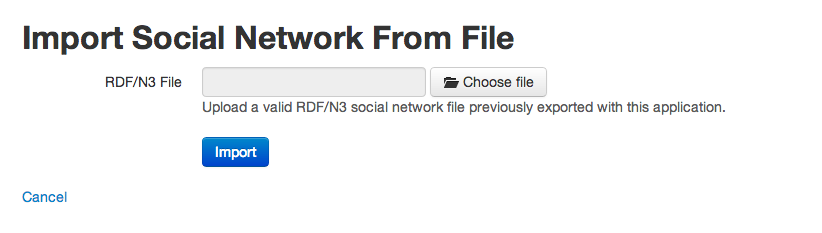
\includegraphics[width=1.0\textwidth]{images/import_sn.png}
  \caption[Importación de una Red Social]{\emph{Importación de una Red Social}. Para archivos RDF/N3 exportados previamente con la aplicación.}
  \label{import_sn}
\end{figure}

Cabe destacar que el contenido N3 de la red social puede no definir las posiciones de los nodos, en caso de un archivo que fue exportado sólo con la estructura de la red, no la información visual y por lo tanto la aplicación asigna las posiciones en base al algoritmo de layout de grafos de Fruchterman-Reingold~\cite{sna}, con lo cual crea los nodos, las familias, roles e interacciones entre ellos según lo especifica el archivo usado.

% section importación_en_rdf (end)

\section{Unión de Redes Sociales} % (fold)
\label{sec:union_de_redes_sociales}

Una de las funcionalidades claves de esta aplicación, que es una mejora con respecto a la experiencia de Manuel Bahamonde~\cite{memoriamanuel}, es la unión de redes sociales, esta consiste en que los datos generados de forma manual con la aplicación pueden ser complementados con datos generados por otros usuarios de la misma.\\

Para unir redes sociales, se utiliza el botón de creación de redes sociales y se elige la opción de unir dos redes sociales, en donde aparece el formulario de unión de redes sociales~\ref{seleccion_union}, en donde inicialmente seleccionamos un archivo RDF/N3 para importar la red, luego seleccionamos a que red se va a unir esta red social importada como indica el formulario de la figura.\\

\begin{figure}[H]
  \centering
  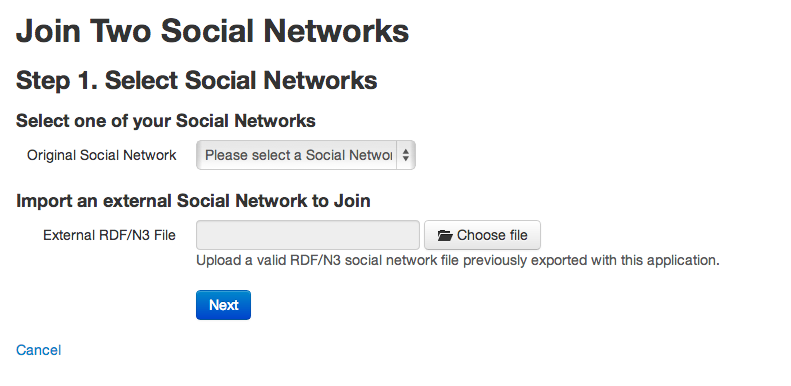
\includegraphics[width=0.6\textwidth]{images/seleccion_union.png}
  \caption[Selección de Redes a Unir]{\emph{Selección de Redes a Unir}. Se selecciona una red social que el usuario posee y se importa una red social externa con la que se va a unir.}
  \label{seleccion_union}
\end{figure}

Luego de presionar \emph{Next} en el formulario de unión, lo siguiente es definir las equivalencias dentro de las familias de ambas redes sociales~\ref{equivalencia_familias}, en donde a cada familia de la red original, selecciono una, más de una o ninguna equivalencia con una familia de la red social importada. Una vez estas equivalencias son definidas, se procesan en el back-end para añadir todos los datos de la red social importada en la seleccionada.\\

\begin{figure}[H]
  \centering
  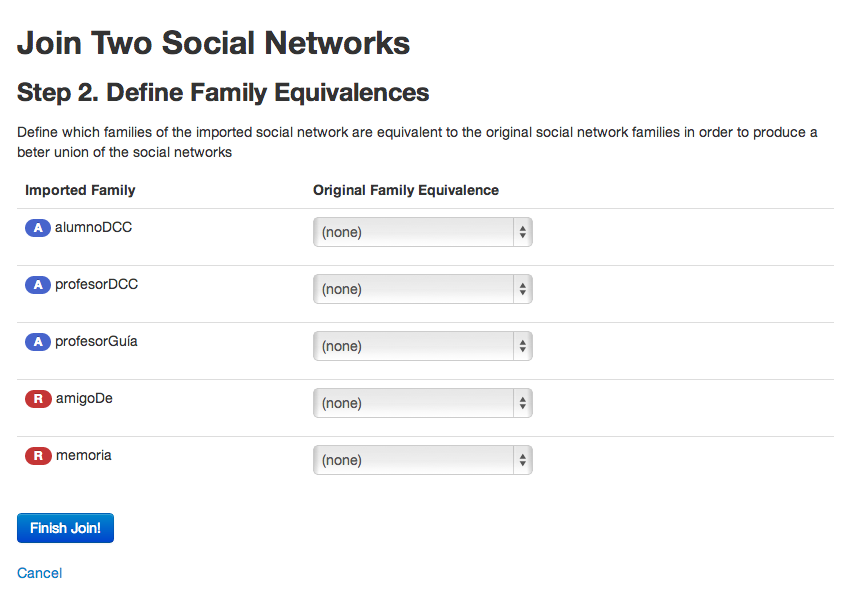
\includegraphics[width=0.7\textwidth]{images/equivalencia_familias.png}
  \caption[Selección de Equivalencias entre Familias]{\emph{Selección de Equivalencias entre Familias}. En esta pantalla se seleccionan que familias de la red importada para unir, son equivalentes a las familias de la red social original, en múltiples equivalencias a la misma familia original son permitidas.}
  \label{equivalencia_familias}
\end{figure}

Con respecto a las relaciones, cabe mencionar que si en una red social está la relación $A$ con familia $F_1$ y en la otra red social se encuentra la relación $B$ con familia $F_2$, al momento de determinar que $F_1 = F_2$, la relación $B$ es eliminada y todos sus roles pasan a la relación $A$ debido a que ambas relaciones se consideran equivalentes

Luego de completar las operaciones anteriores, las redes sociales estarán unidas dentro de la original, donde los nodos fueron reordenados. Lo siguiente es definir las equivalencias entre nodos, para esto se selecciona el modo de unión en el menú de edición~\ref{ssub:modos_de_edicion}, con esto, solo basta arrastrar un nodo sobre otro y confirmar el dialogo que aparece al soltar el nodo para unirlos (figura~\ref{node_join}). Al unir un par nodos se combinan las familias, los atributos y roles de estos, comportamiento el cual se decidió de esta forma debido a que un nodo puede no tener un nombre y su contexto (familias, atributos y nodos) expresan mucho mejor la entidad que representa el nodo y de esta forma visual es más sencillo encontrar la equivalencia entre estos.

\begin{figure}[H]
  \centering
  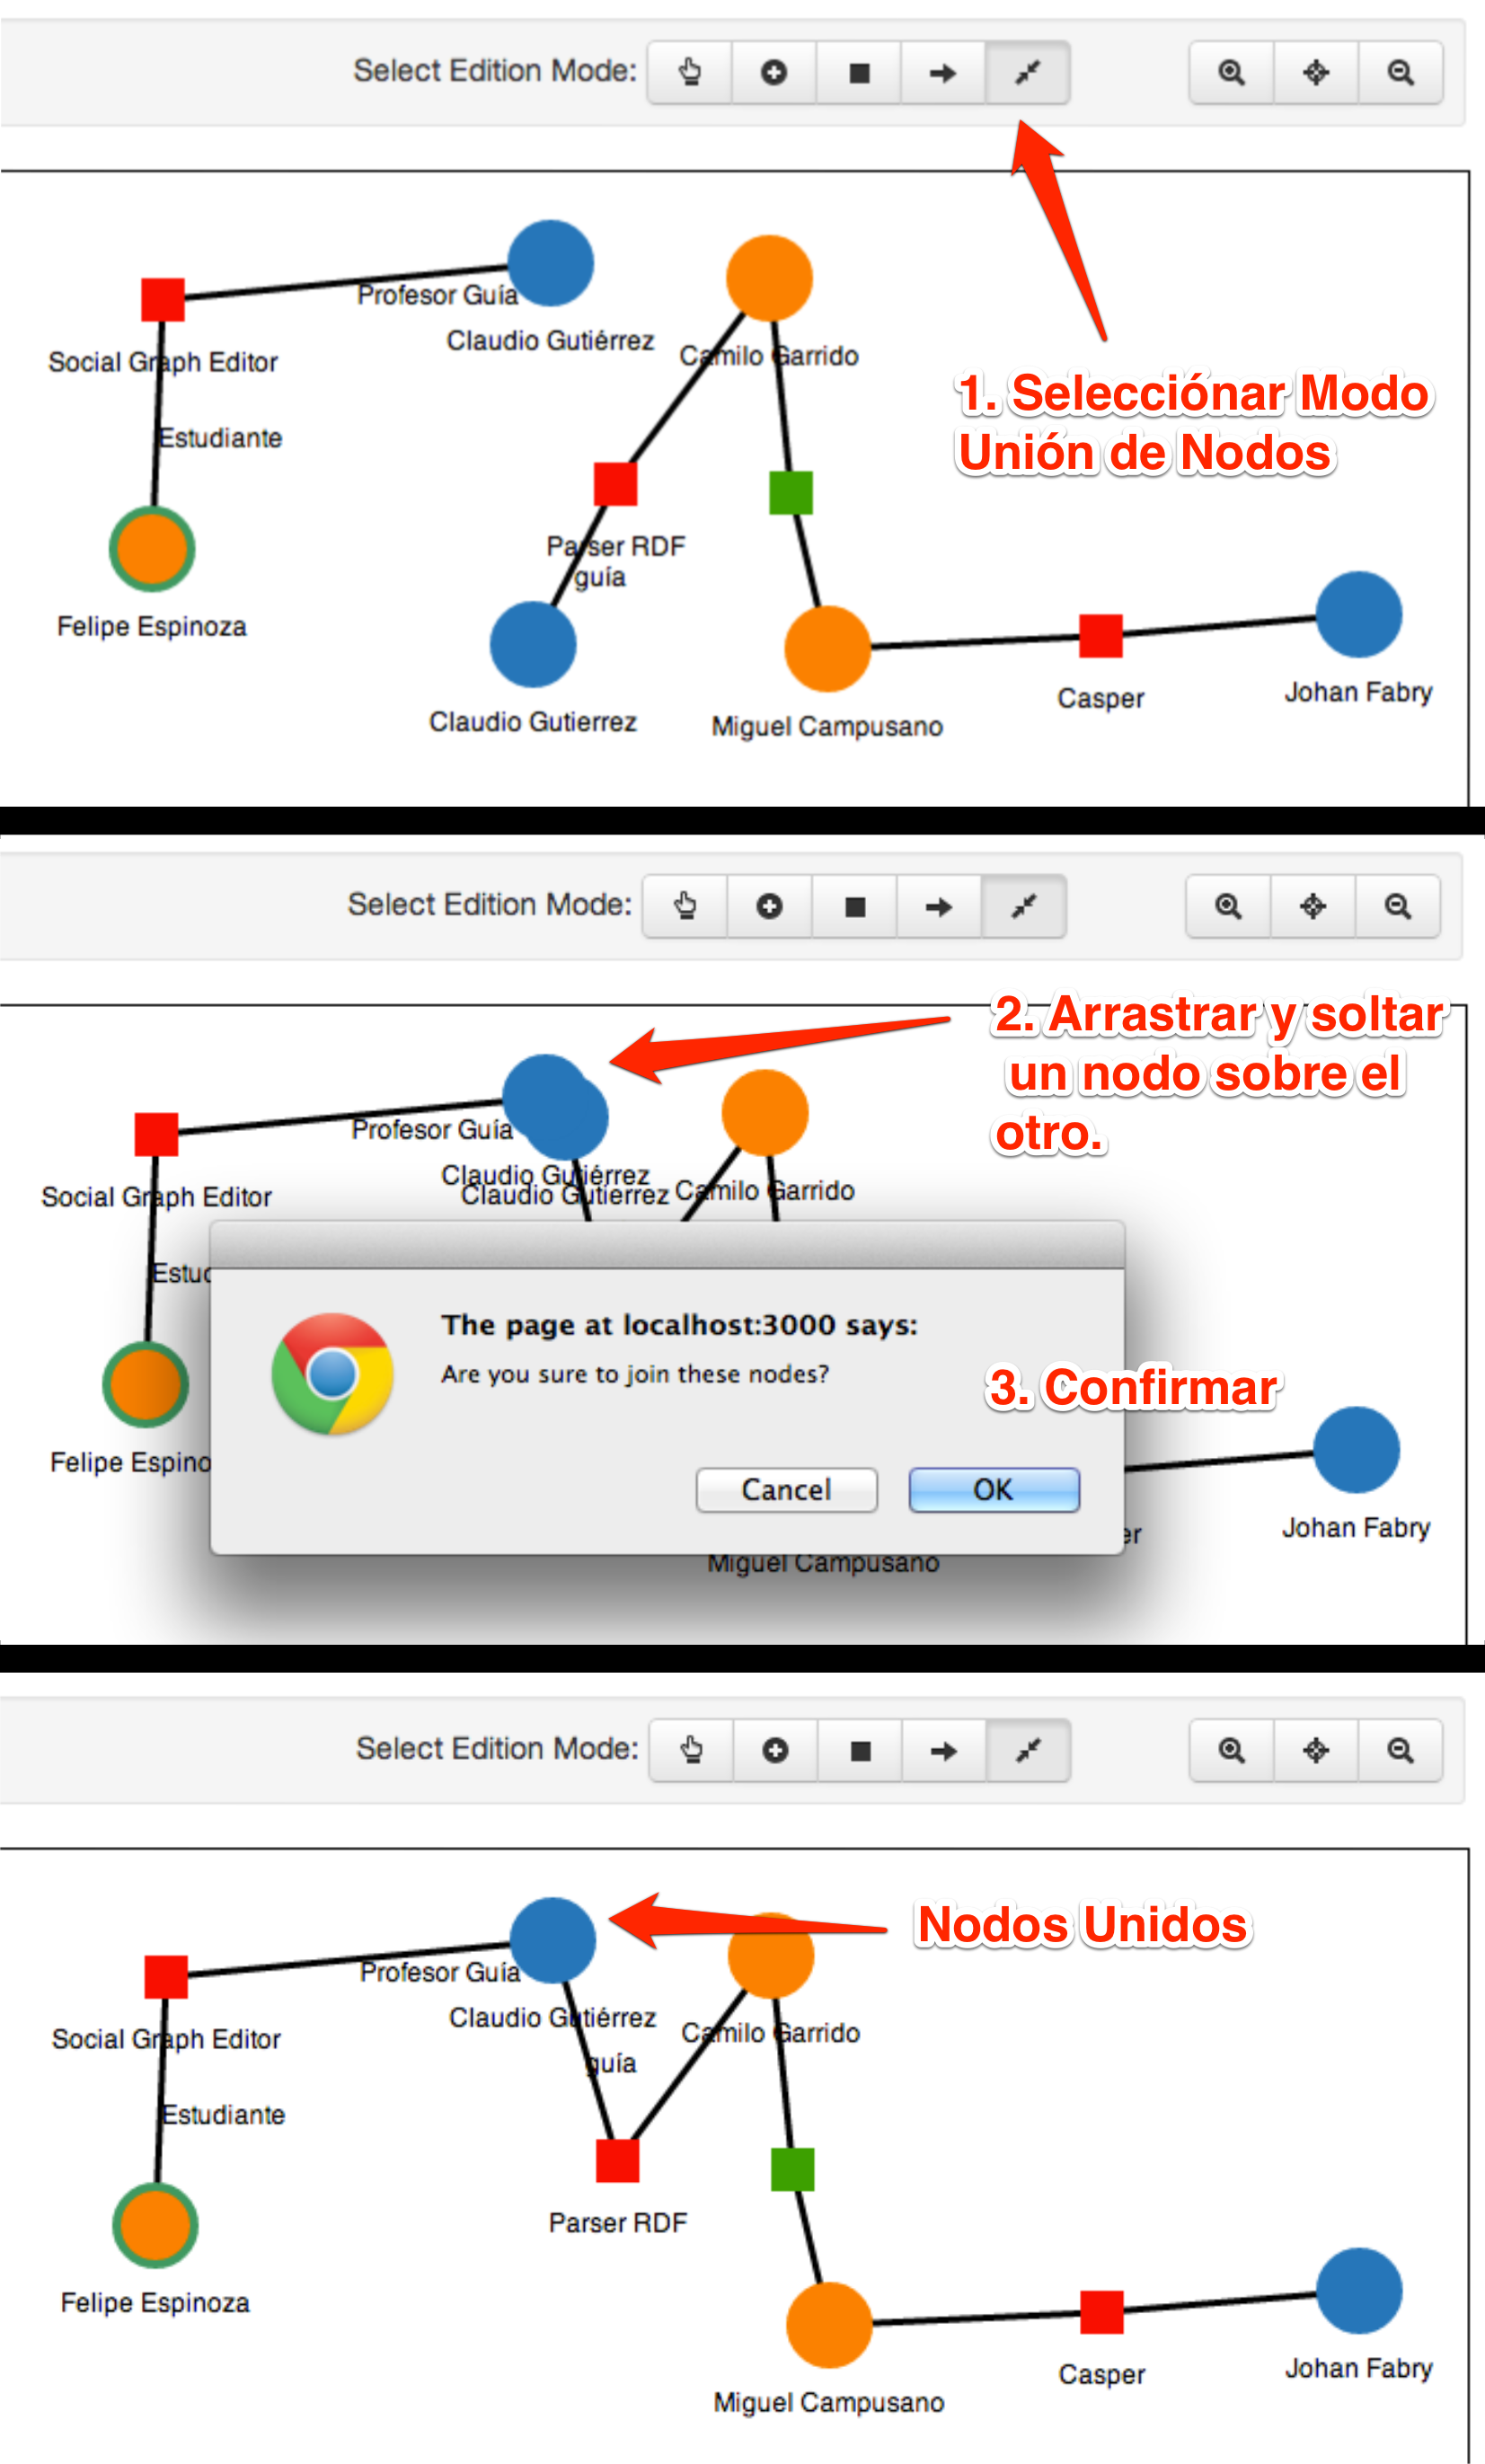
\includegraphics[width=0.7\textwidth]{images/node_join.png}
  \caption[Operación de Unión de Nodos]{\emph{Operación de Unión de Nodos}. Explicación de los 3 pasos para unir dos nodos entre sí (actores o relaciones): seleccionar el modo de unión de nodos, tomar un nodo y arrastrarlo al que se desea unir y confirmar la operación. Con estos pasos se unen los nodos.}
  \label{node_join}
\end{figure}

% section union_de_redes_sociales (end)

\section{Ejemplos de Uso} % (fold)
\label{sec:ejemplos_de_uso}

% El software que se implemento ́ esta disen ̃ado para ser utilizado por investigadores que recopilan sus datos desde varias fuentes. Se asume que estas fuentes dif ́ıcilmente cuentan con toda la informacio ́n, o estas se encuentra en un formato donde no se puede automatizar el proceso de transcribir la informacio ́n desde la fuente original hasta una red social.

% section ejemplos_de_uso (end)
